\documentclass{beamer}
\usepackage[utf8]{inputenc}
\usepackage[final]{pdfpages}
\usetheme{Goettingen}%Warsaw}
\usecolortheme{lily}
\setbeamertemplate{footline}[page number]
\title[Fast classification]{Efficient dynamic and static environment classification in Occupancy Grid framework}
\author{Jander Nascimento}
\institute{Université Joseph Fourier / INRIA}
\date{\today}
\begin{document}

\begin{frame}
\titlepage
\end{frame}

%\AtBeginSubsection[]
{
  \begin{frame}<beamer>
    \frametitle{Roadmap}
    \tableofcontents%[currentsection,currentsubsection]
  \end{frame}
}

\section{Problem}

	\begin{frame}
		\frametitle{Problem overview}
		\begin{figure}[h]
			\center
			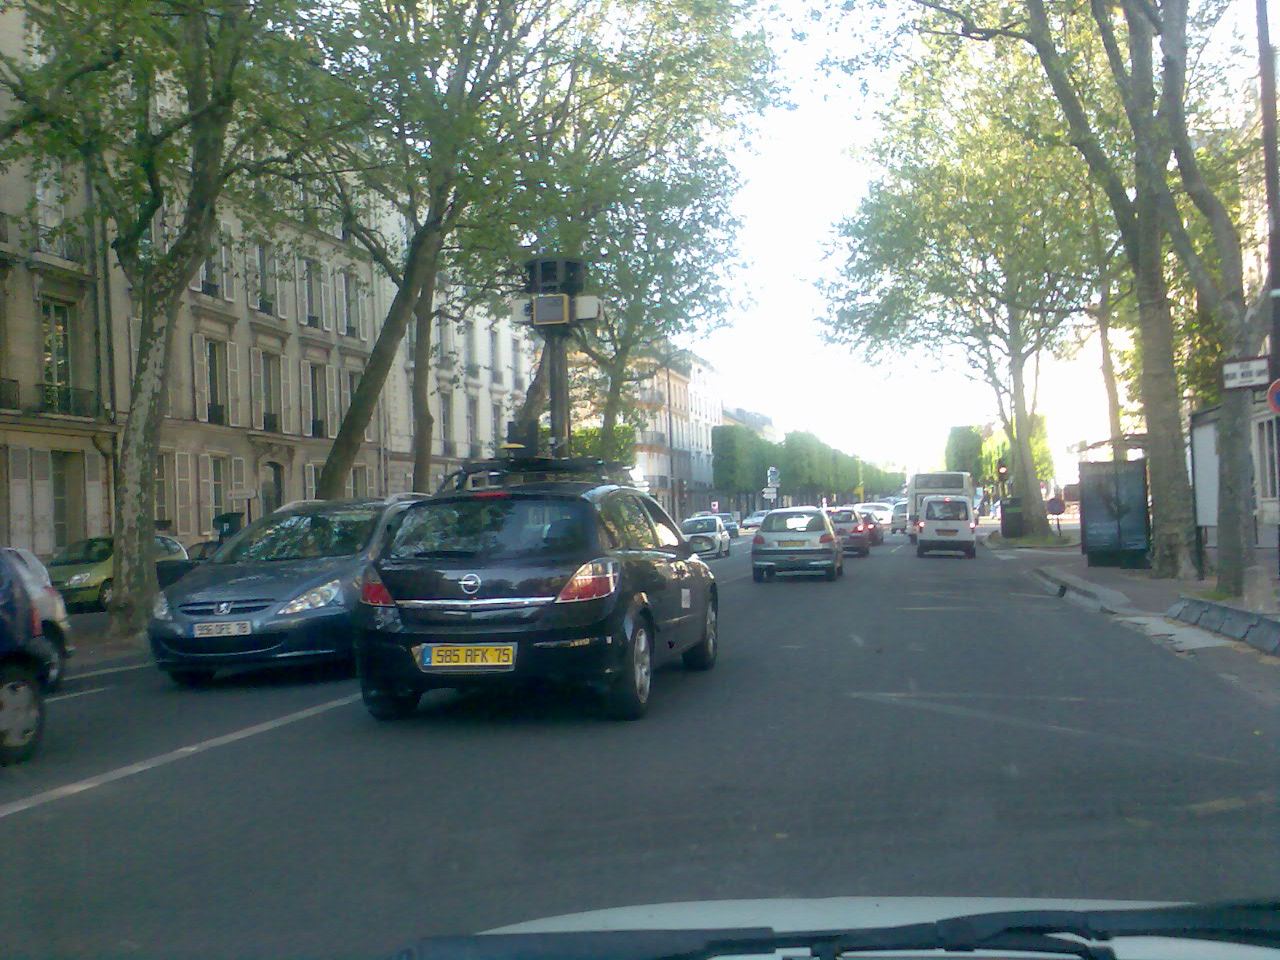
\includegraphics[scale=0.1]{img/fig:street:urban}
		 \end{figure}
		 
		\begin{block}{Problem}
			 Being able to identify the dynamic parts of the environment
		\end{block}
		 
		Constrains
		\begin{itemize}
			\item In a car (platform)
			\item using a laser scanner (sensor)
			\item As fast as possible (online)
		\end{itemize}

		\begin{alertblock}{Not our goal}
			solve DATMO and SLAM
		\end{alertblock}
	\end{frame}


\section{Introduction}

\subsection{Intelligent Transportation Systems}

	\begin{frame}
		\frametitle{ITS overview}
	
		\begin{figure}[h]
			\center
			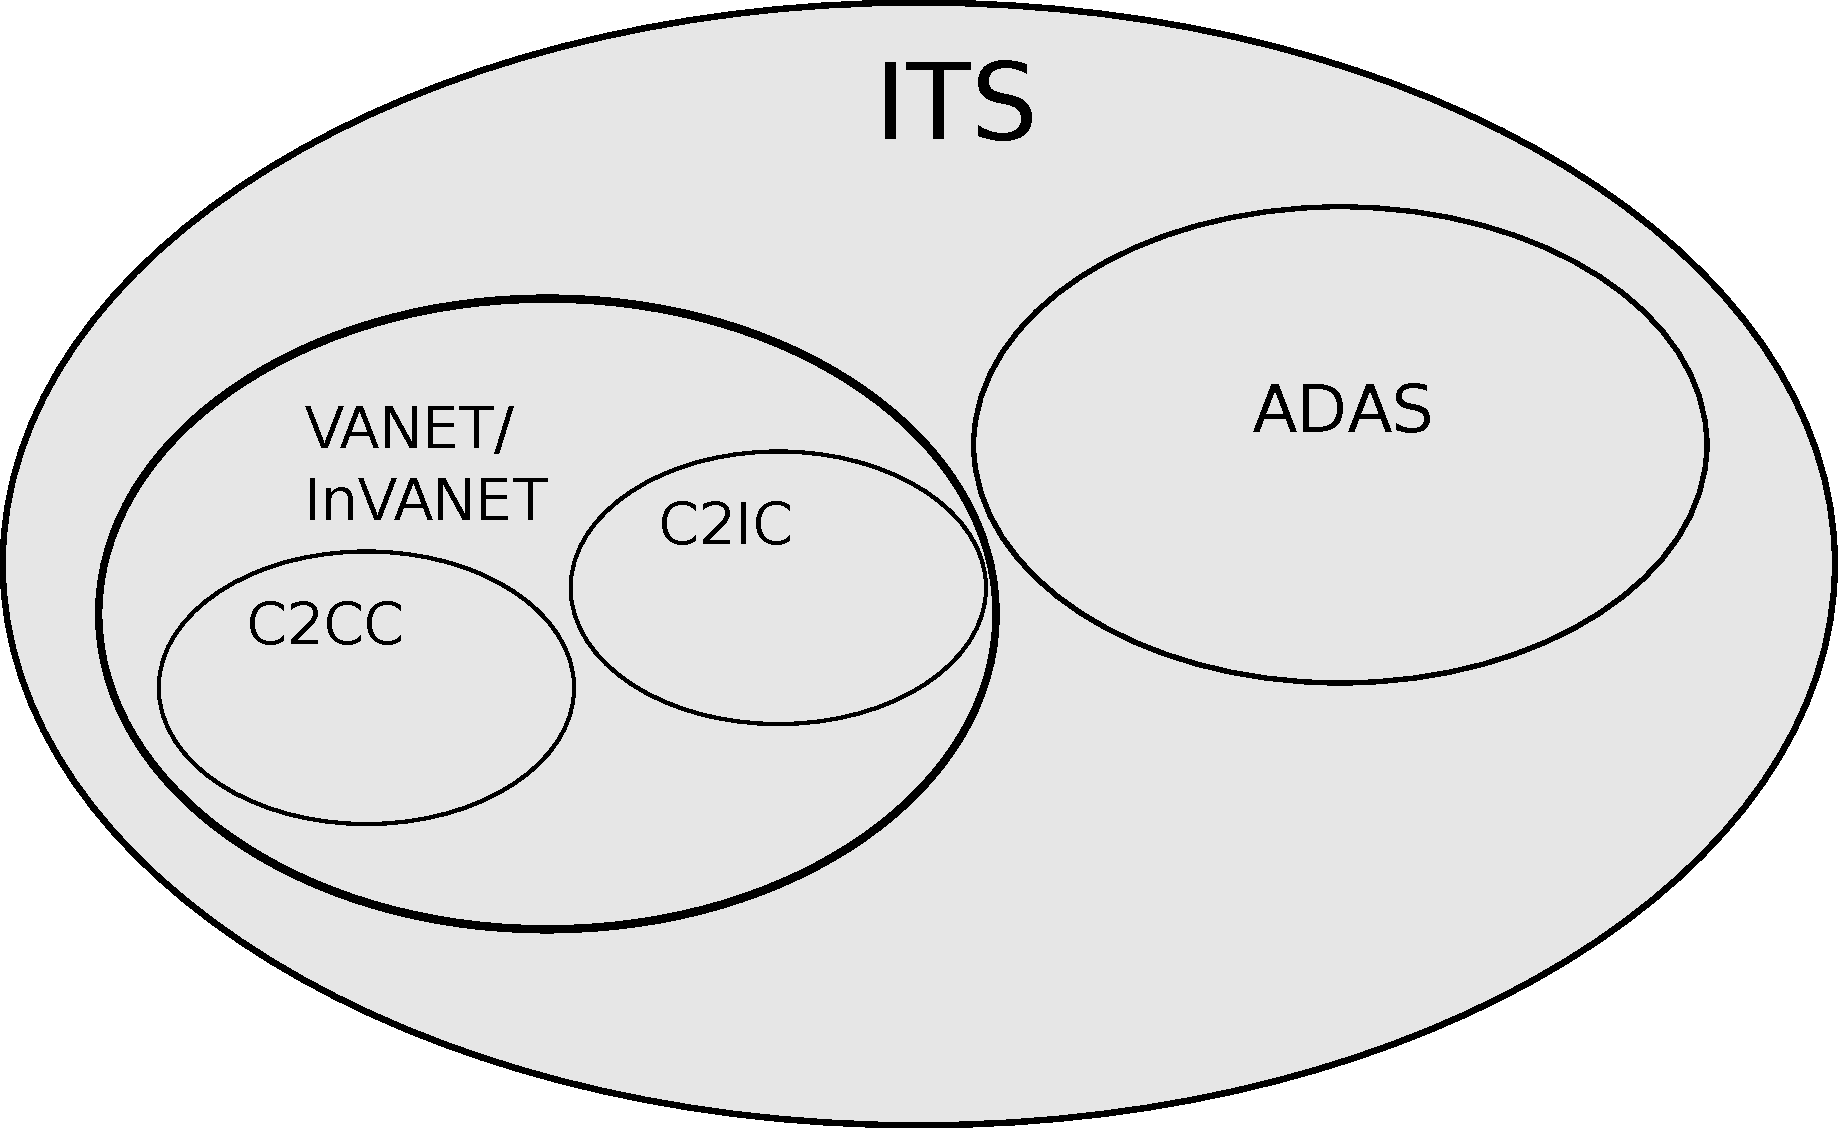
\includegraphics[scale=0.3]{img/fig:its:division}
		 \end{figure}		
		
	\end{frame}

	\begin{frame}
		\frametitle{ADAS}
		\begin{exampleblock}{Stands for}	
			Advanced Driver Assistance Systems		
		\end{exampleblock}				
		\begin{block}{Canonical definition}
			Cope with vehicle handling tasks
		\end{block}		

		\begin{block}{Goal}
			\begin{itemize}
			\item Reduce the risk of collisions
			\item Reduce the driver overload
			\item Increase the confort
			\end{itemize}
		\end{block}
		
	\end{frame}

\subsection{Sensors}

	\begin{frame}
		\frametitle{Sensor overview}
	
		\begin{block}{Canonical definition}
			Translate physical \textit{stimuli} in electronic information
		\end{block}
	
		Classified according to?	
		\begin{block}{Definition}
			\begin{itemize}
			\item measurand observed
			\item subject's localization
			\item technology used
			\end{itemize}
		\end{block}			
	
	\end{frame}

	\begin{frame}
		\frametitle{Measurand observed}
		Which kind of physical \textit{stimulus} can be observed?
		\begin{figure}[h]
			\center
			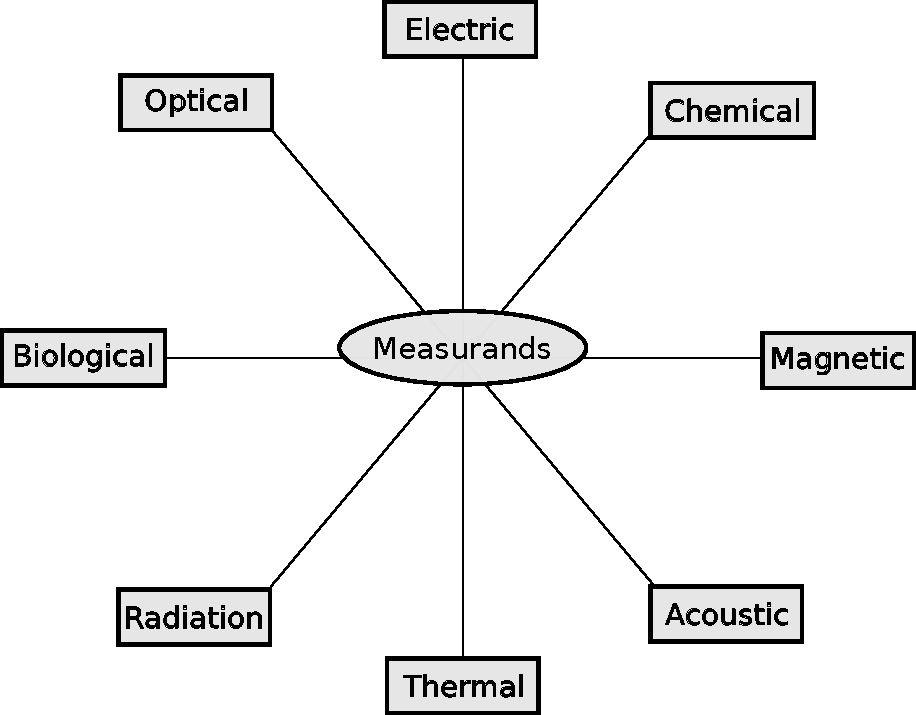
\includegraphics[scale=0.4]{../img/fig:sensors}
		 \end{figure}				
	\end{frame}
	
	\begin{frame}
		\frametitle{subject's localization}
		What we are observing belongs to the moving robot?
		\begin{itemize}
		\item Yes! proprioceptive
		\item No! exteroceptive
		\end{itemize}
		\begin{figure}[h]
			\center
			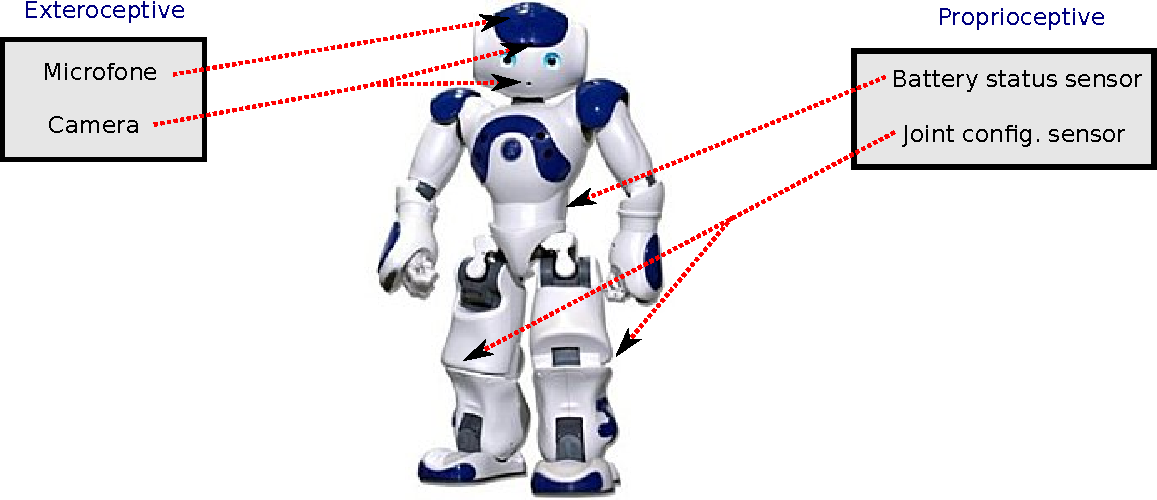
\includegraphics[scale=0.4]{img/fig:nao:config}
		 \end{figure}		
	\end{frame}

	\begin{frame}
		\frametitle{technology used}
		\begin{itemize}
		\item passive
			\begin{itemize}
				\item Emits energy to the enviroment so the measurand can be obtained
				\item e.g. range sensor, radars, etc.
			\end{itemize}		
		\item active
			\begin{itemize}
				\item Receives a physical info and is able to deduce the measurand
				\item e.g. camera, microfone, etc. 
			\end{itemize}		
		\end{itemize}		
		
	\end{frame}
	
	\begin{frame}
		\frametitle{What can we said about them?}

		\begin{itemize}
			\item Imprecision
			\item Uncertainty
			\item Incomplete data
		\end{itemize}		
		
	\end{frame}

\section{Perception process}

	\begin{frame}
		\frametitle{Perception overview}
		\begin{block}{Definition}
			The process of acquiring knowledge about the environment \cite{iyengar1991autonomous}
		\end{block}	
		
		\begin{figure}[h]
			\center
			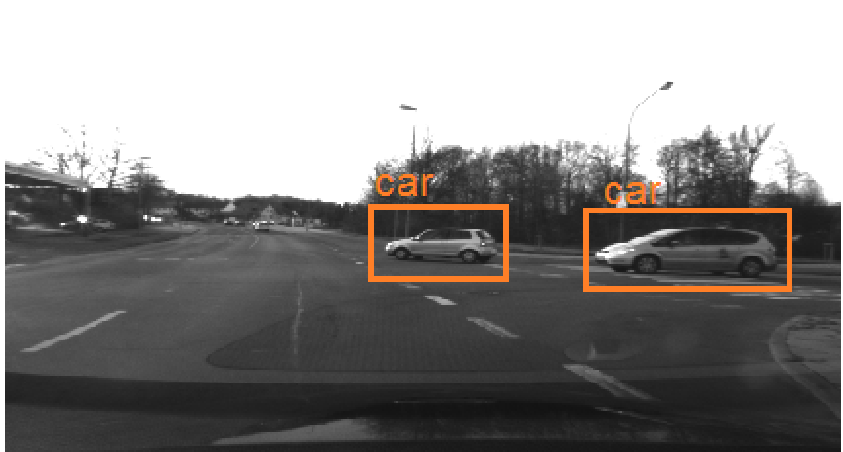
\includegraphics[scale=0.3]{img/fig:perception:ex1}
		\end{figure}
		 
	\end{frame}

	\begin{frame}
		\frametitle{Perception frequent terms}

		\begin{itemize}
			\item Mapping
			\item Localization
			\item Detection
			\item Tracking
		\end{itemize}				

	\end{frame}

	\begin{frame}
		\frametitle{Grouping process in robotics}
		
		\begin{block}{Goal}		
			Dependable informations are grouped in the same process.
		\end{block}			
		
		\begin{exampleblock}{Process}		
		
			\begin{itemize}
			\item Localization
			\item Mapping
			\end{itemize}			
		
			SLAM
		\end{exampleblock}					
				
		\begin{exampleblock}{Process}		
			\begin{itemize}
			\item Moving objects
				\begin{itemize}
				\item Detection
				\item Tracking
				\end{itemize}			
			\end{itemize}			
			DATMO
		\end{exampleblock}						
				
	\end{frame}

	\subsection{SLAM}
		\begin{frame}
			\frametitle{SLAM}
			
			\begin{block}{Stands for}				
				Simultaneous Localization and Mapping
			\end{block}
			
			\begin{quotation}
				Providing the vehicle with a map of static parts of the environment as well as its location in the map \cite{DBLP:journals/inffus/VuBA11}
			\end{quotation}			
			
			\begin{figure}[h]
				\center
				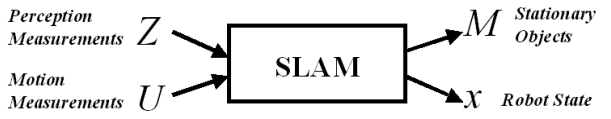
\includegraphics[scale=0.8]{../img/fig:perception:slam}
			 \end{figure}			
			
		\end{frame}
	
	\subsection{DATMO}
		\begin{frame}
			\frametitle{DATMO}
			\begin{block}{Stands for}				
				Detection and Tracking of Moving Objects
			\end{block}
			\begin{quotation}
				being aware of dynamic entities around, tracking them, and knowing their future position\cite{DBLP:journals/inffus/VuBA11}
			\end{quotation}				
			\begin{figure}[h]
				\center
				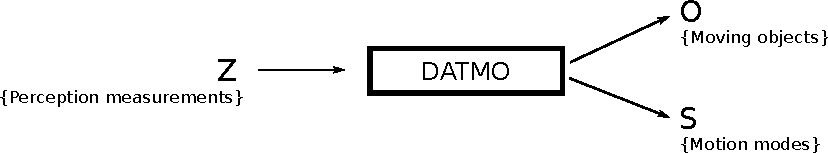
\includegraphics[scale=0.8]{../img/fig:datmo:process}
			 \end{figure}		
		\end{frame}

%%%%%%%%%%%%%%%%%%%%%%%%%%%%%%%%%%%%%

\section{State of the art}

	\begin{frame}
		\frametitle{State of the art}
		
		\begin{block}{Mono-vision}
			\begin{itemize}
			\item "Use a Single Camera for Simultaneous Localization And Mapping with  Mobile Object Tracking in dynamic environments" by Migliore et al.
			\item Track MO and Localize with mono-vision (MonoSlam)
			\item Concept
				\begin{itemize}			
				\item Uses a "shadow filter" to classify static features and localize
				\item Initialization features (absence of odometer)
				\item EKF for tracking, with two models
				\item Classifier based on SPRT, optical flow to separate D and S				
				\end{itemize}		
			\item Evaluation results
				\begin{itemize}			
				\item problematic with small displacements
				\end{itemize}	
			\end{itemize}		
		\end{block}
	\end{frame}
	
	\begin{frame}
		\frametitle{State of the art}	
		\begin{block}{Stereo-vision}
			\begin{itemize}
			\item "Mapping in dynamic environments using stereo vision" by Henning Lategahn et al.
			\item Separate static and dynamic parts
			\item Concept
				\begin{itemize}			
				\item Complement occupancy grid + tracking
				\item Disparity image to find the contour
				\item EKF for tracking, with two models
				\item Classifier based on SPRT, optical flow to separate D and S				
				\end{itemize}		
			\item Evaluation results
				\begin{itemize}			
				\item min $2$ max $19$ frames
				\end{itemize}							
			\end{itemize}				
		\end{block}
	\end{frame}

	\begin{frame}
		\frametitle{State of the art}	
		\begin{block}{Laser scanner, Radar and IMU}
			\begin{itemize}
			\item "Grid-based localization and local mapping with moving object detection and tracking" by Trung-Dung Vu et al.
			\item Separate static and dynamic parts
			\item Concept
				\begin{itemize}			
				\item MHT + IMM
				\item 
				\end{itemize}		
			\item Evaluation results
				\begin{itemize}			
				\item min $2$ max $19$ frames
				\end{itemize}				
			\end{itemize}				
		\end{block}
	\end{frame}

\section{Motion Detection}

	\begin{frame}
		\frametitle{Solution overview}
		\begin{figure}[h]
			\center
			\includegraphics[scale=0.5]{img/fig:problem}
		 \end{figure}
		 
		\begin{block}{Problem}
			 Being able to identify the dynamic parts of the environment
		\end{block}
		 
		\begin{block}{Result}
			High level classification
		\end{block}				 

		\begin{alertblock}{Not our goal}
			solve DATMO and SLAM
		\end{alertblock}
	\end{frame}

\subsection{preprocessing}

	\begin{frame}
		\frametitle{Experimental Platform}
		\begin{figure}[h]
			\center
			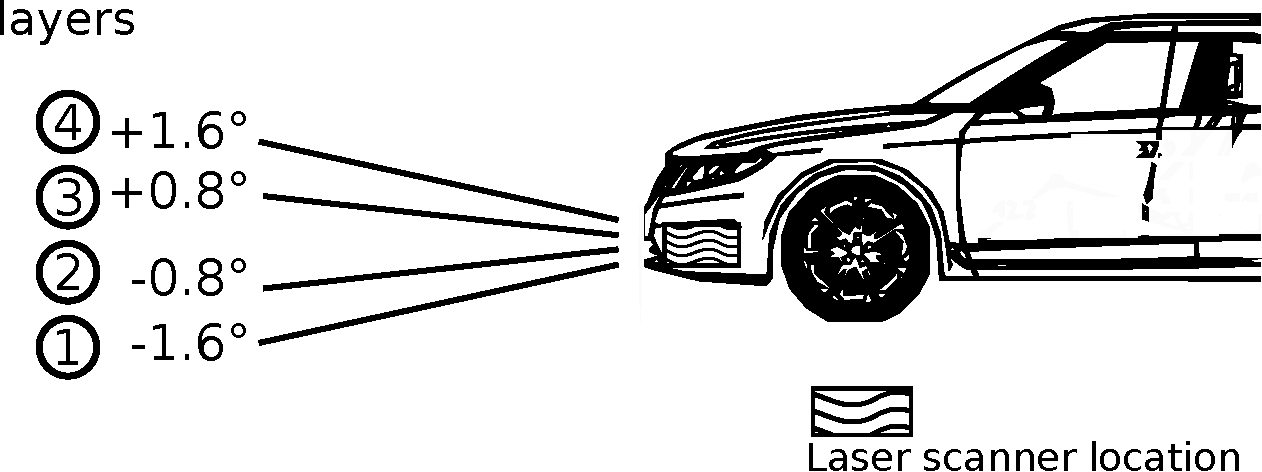
\includegraphics[scale=0.4]{../img/fig:demonstrator:lateral}
		\end{figure}
	\end{frame}

	\begin{frame}
		\frametitle{Experimental Platform}	
		 \begin{columns}[t]
		  \begin{column}{5cm}
		  \begin{figure}[h]
			\center
			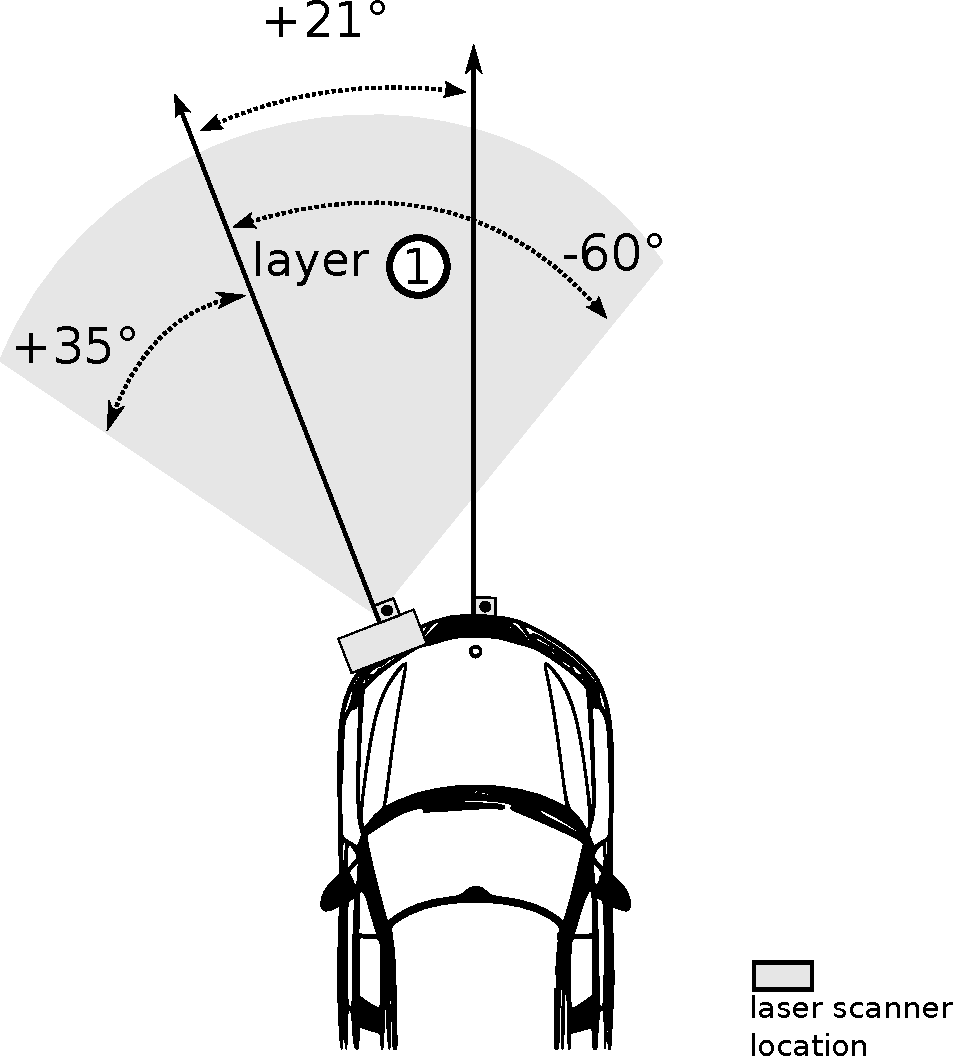
\includegraphics[scale=0.3]{../img/fig:demonstrator:superior}
		  \end{figure}
		  \end{column}
		  
		  \begin{column}{5cm}
		  \begin{figure}[h]
			\center
			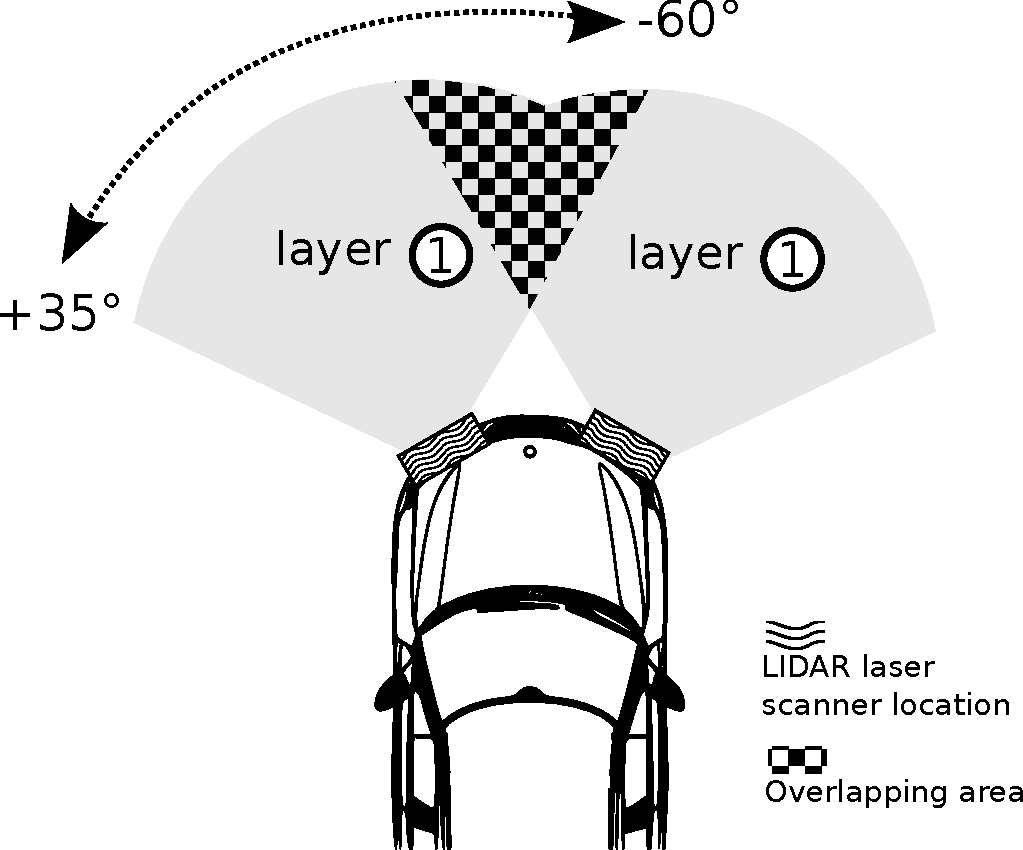
\includegraphics[scale=0.3]{../img/fig:demonstrator:superior:overlap}
		  \end{figure}   
		  \end{column}
		 \end{columns} 	
	
	\end{frame}

	\begin{frame}
		\frametitle{Experimental Platform}
		\begin{figure}[h]
			\center
			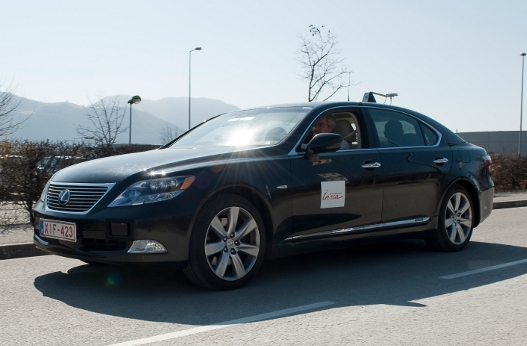
\includegraphics[scale=0.8]{../img/testbed:car}
		  \end{figure}		
		
		  \begin{columns}[t]
		  \begin{column}{5cm}
		  \begin{figure}[h]
			\center
			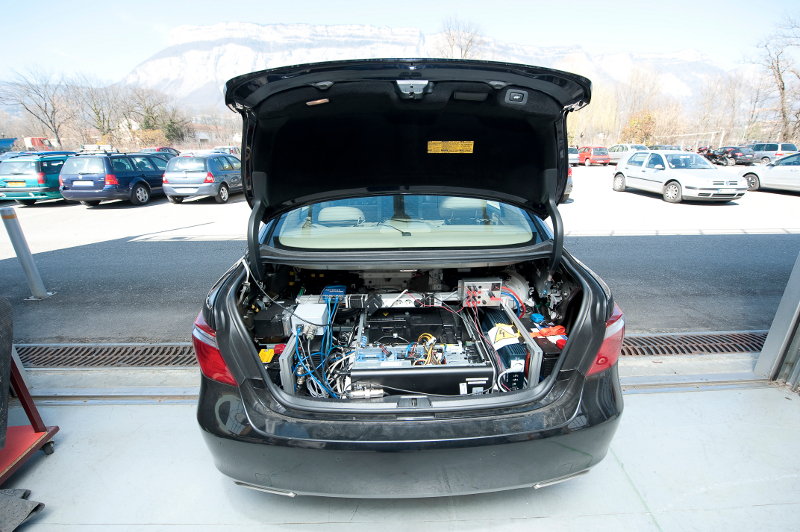
\includegraphics[scale=0.7]{../img/testbed:trunc}
		  \end{figure}
		  \end{column}
		  
		  \begin{column}{5cm}
		  \begin{figure}[h]
			\center
			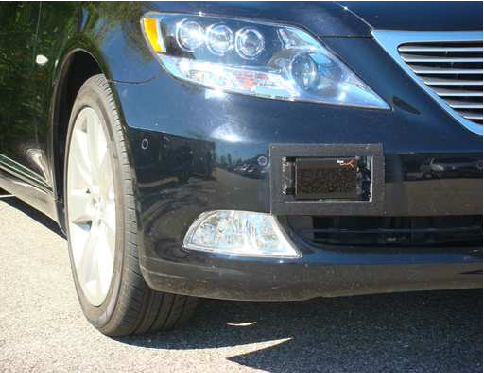
\includegraphics[scale=0.26]{../img/testbed:ibeo}
		  \end{figure}   
		  \end{column}
		 \end{columns}		 
	\end{frame}	

	\begin{frame}
		\frametitle{Input preparation}
		\begin{figure}[h]
			\center
			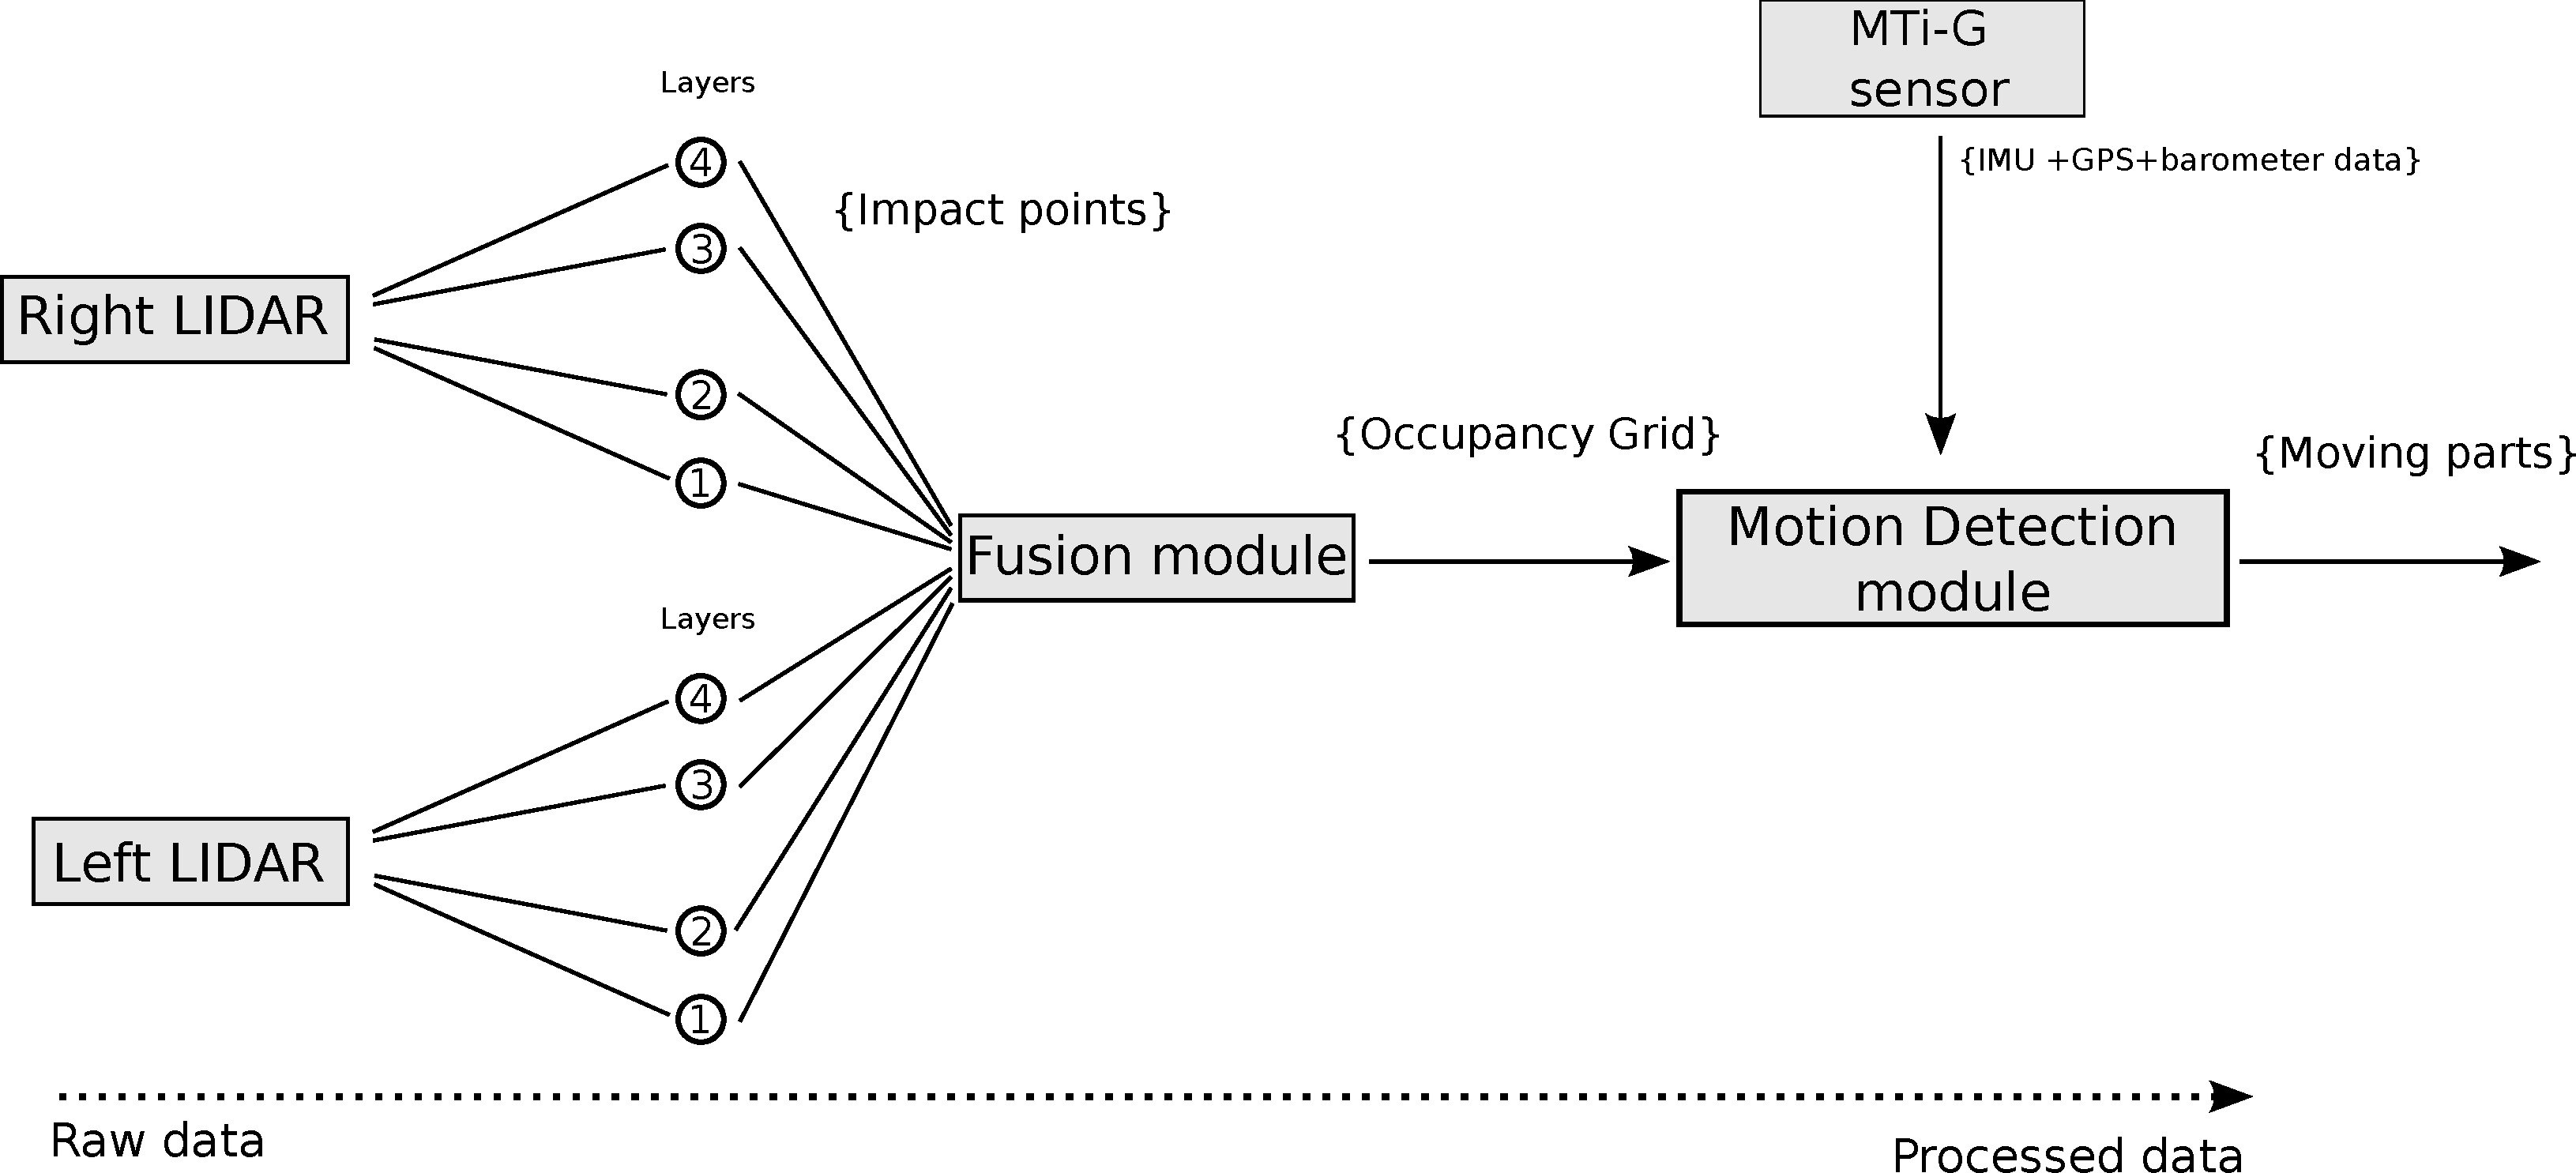
\includegraphics[scale=0.18]{../img/fig:motion:framework}
		\end{figure}
	
		*Linear Opinion Pools \cite{ADARVE-2012-671211}
	
	\end{frame}



	\begin{frame}
		\frametitle{Solution overview}
		\begin{figure}[h]
			\center
			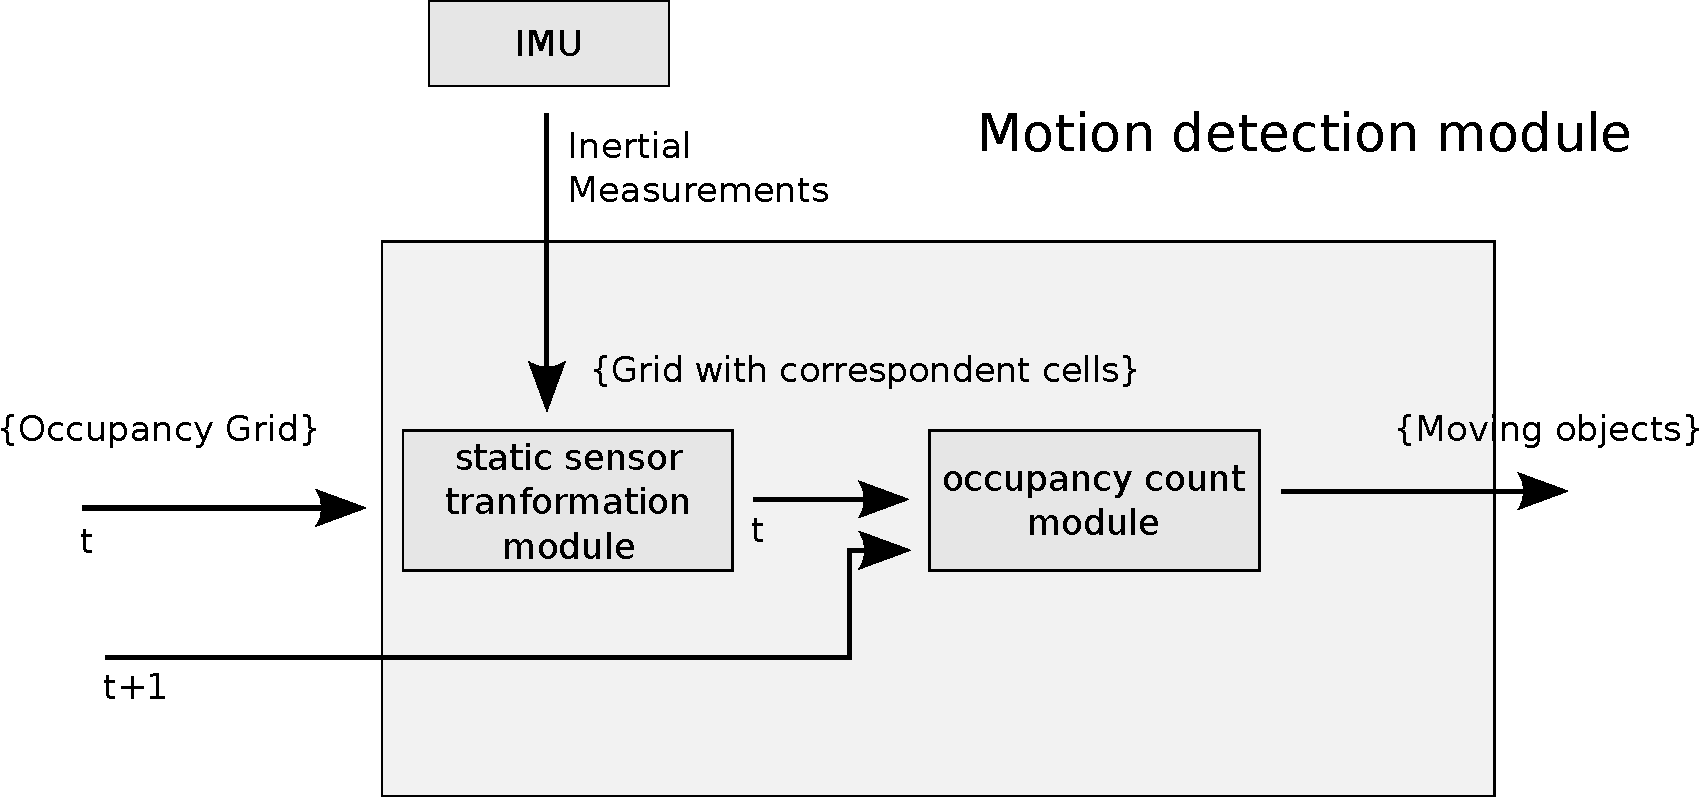
\includegraphics[scale=0.27]{../img/fig:motion:framework:motionmodule}
		 \end{figure}
		
	\end{frame}		
	

\subsection{algorithm}

%%%%%%%%%%%%%%%%%%%%%%%%%%%%%

\section{Experiments}

	\begin{frame}
		\frametitle{Use cases}
		4 use cases were chosen to assess our algorithm:
		\begin{itemize}
		\item Two vehicles, low speed
		\item Two vehicles, at high speed
		\item Vehicle on a roundabout
		\item Complete static scenario
		\end{itemize}						
	\end{frame}

\section{Results}

	\begin{frame}
		\frametitle{Run time}

		\begin{alertblock}{Performance}
			Run in approximately 3.0ms in a 2.67Mhz processor
		\end{alertblock}		
		
		\begin{exampleblock}{Bright side}
			Still place for optimization
		\end{exampleblock}				
		
	\end{frame}	

	\begin{frame}
		\frametitle{Two vehicles, low speed}
		%image
		\begin{exampleblock}{Positive}
		\begin{itemize}
		\item Visibility
		\end{itemize}
		\end{exampleblock}
						
		\begin{alertblock}{Negative}
		\begin{itemize}
		\item False positive (Bottom-right side)
		\end{itemize}
		\end{alertblock}					

		\begin{block}{Reason?}
		Bad rotation velocity data (IMU)
		\end{block}
		
	\end{frame}
	\begin{frame}
		\frametitle{Two vehicles, at high speed}
		%image
		\begin{exampleblock}{Positive}
		\begin{itemize}
		\item Good results at high speed (when its most needed)
		\end{itemize}
		\end{exampleblock}
						
		\begin{alertblock}{Negative}
		\begin{itemize}
		\item False positive (Middle part of the image)
		\end{itemize}
		\end{alertblock}					

		\begin{block}{Reason?}
		Bad rotation velocity data (IMU)
		\end{block}		
	\end{frame}
	
	\begin{frame}
		\frametitle{Vehicle on a roundabout}
		%image
		\begin{exampleblock}{Positive}
		\begin{itemize}
		\item Very dense pixels
		\end{itemize}
		\end{exampleblock}
						
		\begin{alertblock}{Negative}
		\begin{itemize}
		\item False positive 
		\end{itemize}
		\end{alertblock}					

		\begin{block}{Reason?}
		Bad rotation velocity data (IMU)
		\end{block}			
	\end{frame}
	\begin{frame}
		\frametitle{Complete static scenario}
		%image
		\begin{exampleblock}{Positive}
		\begin{itemize}
		\item Only few sparse pixels
		\end{itemize}
		\end{exampleblock}
						
		\begin{alertblock}{Negative}
		\begin{itemize}
		\item False positive
		\end{itemize}
		\end{alertblock}					

		\begin{block}{Reason?}
		Bad rotation velocity data (IMU)
		\end{block}			
		
	\end{frame}			

	\begin{frame}
		\frametitle{Conclusion - Pros and Cons}
		
		\begin{block}{Pros}
			\begin{itemize}
			\item easy to integrate with existing solutions
			\item faster way to classify
			\end{itemize}
		\end{block}		
		
		\begin{block}{Cons}
			\begin{itemize}
			\item Need to be filtered after all to reduce the noise
			\item Sensible to IMU data precision
			\end{itemize}
		\end{block}
		
	\end{frame}

%\begin{thebibliography}{9}
%	\begin{frame}{References}
%		\bibitem{iyengar1991autonomous}
%			Iyengar, S.S. and Elfes, A.
%			\emph{Autonomous Mobile Robots: Control, planning, and architecture}.
%			1991.
%			
%		\bibitem{DBLP:journals/inffus/VuBA11}
%			Trung-Dung Vu, Julien Burlet, Olivier Aycard
%			\emph{Grid-based localization and local mapping with moving object
%              detection and tracking}.
%			2011.			
%
%		\bibitem{hal-00671211}
%			Adarve, Juan David and Perrollaz, Mathias and Makris, Alexandros and Laugier, Christian
%			\emph{Computing Occupancy Grids from Multiple Sensors using Linear Opinion Pools}.
%			2012.
%
% 	\end{frame}
%	\end{thebibliography}

	\begin{frame}{This is the end..}
	\begin{alertblock}{}
		\center
		Questions?
	\end{alertblock}
	\end{frame} 	
 	
\bibliographystyle{abbrvnat}
\bibliography{../report}{} 	
 	


\end{document}